\documentclass[tikz,border=0pt]{standalone}
\usepackage{graphicx}
\usepackage{helvet}
\renewcommand{\familydefault}{\sfdefault}
\begin{document}
\begin{tikzpicture}[x=1mm,y=1mm]
  \node[anchor=south west,inner sep=0] at (0,0)
    {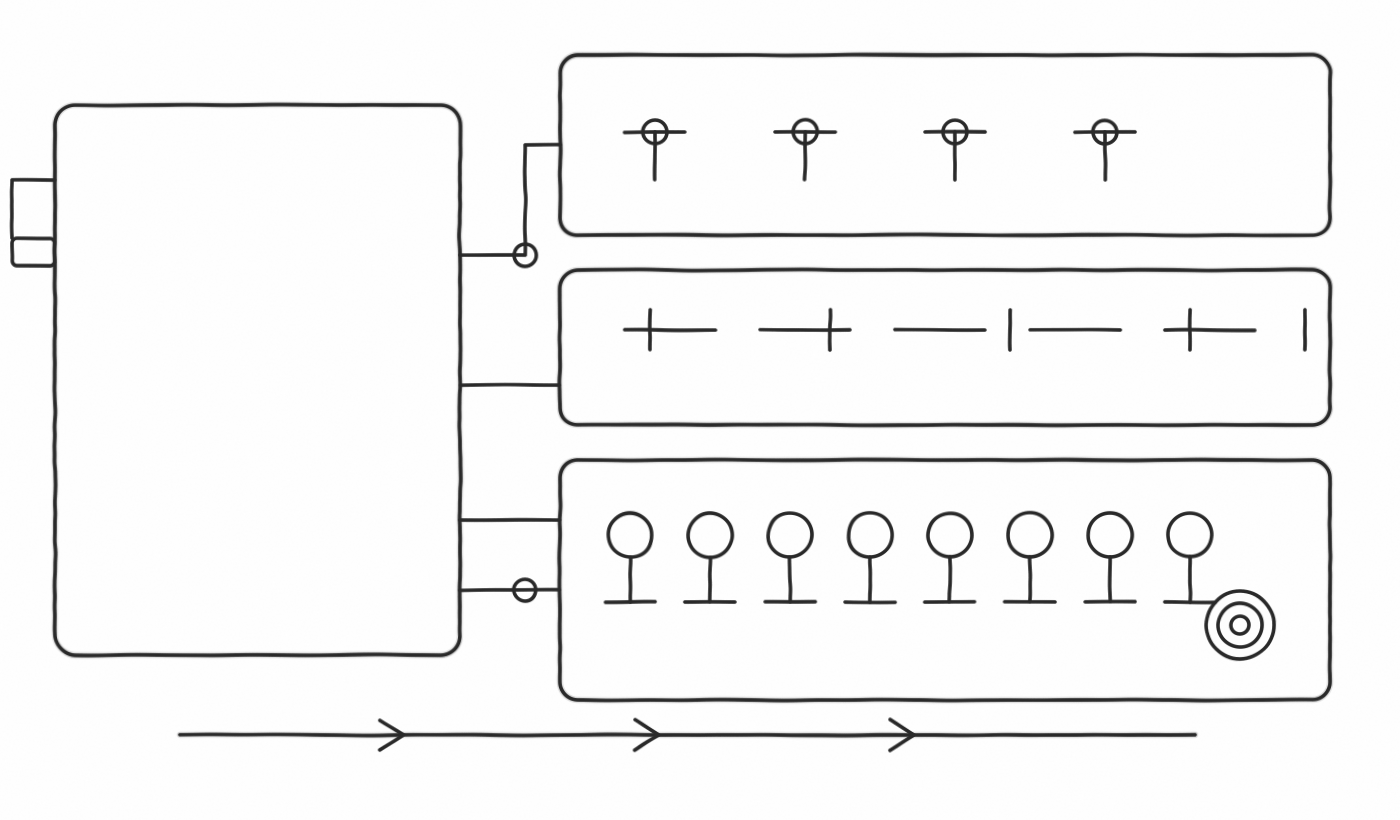
\includegraphics[width=140mm,height=82mm]{030-inert-show-pencil-base.png}};
  \node[font=\bfseries\large] at (25.8,66) {MEGA 2560};
  \node[font=\small] at (25.8,61.5) {USB 5 V only};
  \node[font=\small] at (25.8,51) {D35--D38 synthetic editor};
  \node[font=\small] at (25.8,46.5) {D30--D34 operator buttons};
  \node[font=\small] at (25.8,42) {D22--D29 cue LEDs};
  \node[font=\small] at (25.8,37.5) {D5--D7 RGB state};
  \node[font=\bfseries\small] at (94.5,72.5) {SYNTHETIC OBSERVATION EDITOR};
  \foreach \x/\t in {65.5/CHANNEL,80.5/PRIMARY,95.5/REDUNDANT,110.5/APPLY}
    \node[font=\tiny] at (\x,61) {\t};
  \node[font=\tiny] at (51.5,57) {TP28};
  \node[font=\bfseries\small] at (94.5,51.5) {OPERATOR BUTTONS TO GND};
  \foreach \x/\t in {65/REVIEW,83/RUN,101/CONFIRM,119/SKIP,130.5/CANCEL}
    \node[font=\tiny] at (\x,43) {\t};
  \node[font=\bfseries\small] at (94.5,35.5) {EIGHT CUE LEDs -- 1 kOhm EACH};
  \foreach \x/\n in {63/0,71/1,79/2,87/3,95/4,103/5,111/6,119/7}
    \node[font=\tiny] at (\x,17.5) {\n};
  \node[font=\tiny] at (124,13.5) {RGB STATE};
  \node[font=\tiny] at (51.5,23) {TP29};
  \foreach \x/\t in {28/observe,53/assess,78.5/review + confirm,105/inert cue + audit}
    \node[font=\scriptsize] at (\x,3.5) {\t};
\end{tikzpicture}
\end{document}
